Successful operation of modern networked computer systems are not by coincidence or luck.
Network operators heavily relies on the realistic and scalable testing platforms to
evaluate the functionality and the performance of their communication infrastructures and protocols.
Moreover, as the successfully and widely deployed computer networking technology gets deeply integrated into people's everyday lives,
it is no longer optional to protect network against cyber-attacks.
Occurred attacks should be thoroughly studied and its defense carefully implemented to ensure safe and trusted communication of information.
Replaying the attacks happened in real world and, more importantly, practicing, as well as evaluating, the countermeasures become 
enormously difficult if without a virtually simulated or emulated testbed.
Meanwhile, the network today in many domains and settings, are evolving toward the software-defined networking (SDN) paradigm.
SDN promises centralized and rapid network provisioning, holistic management, low operational cost, and improved network visibility.
Multiple SDN simulation and emulation platforms have help expedite the adoption of many emerging SDN-based applications to production systems.
However, all of those virtual simulation or emulation testbeds are highly coupled with the underlying available physical hardware resources.
As the result, their correctness will be corrupted, their scalability limited, and their fidelity compromised,
especially exposed under the common large-scale network settings.
Under the centre theme of securing SDN-enabled large-scale network using high-fidelity and scalable testing system, our research work has three streams.

\Section{Virtual Time Support for Network Emulation}
\label{VT:Sec:Intro}

Linux-container-based network emulation (LCNE) combines many desired features of software simulators and physical testbeds.
Therefore, we first ask not what LCNE can do for computer network, but ask what we can do for LCNE.
Specifically, we address one of the key issues of this attractive methodology.
An ordinary Linux-container-based SDN emulator uses the system clock across all the containers even if a container is not being scheduled to run.
This leads to the issue of both performance and temporal fidelity, especially when handling high workloads during emulation.

Our approach is to develop the notion of virtual time inside containers to improve fidelity and scalability of the container-based network emulation.
A key insight is to trade time for system resources by precisely scaling the system's capacity to match behaviors of the target network.
The idea of virtual time has been explored in the form of time-dilation-based~\cite{ToInfinityBeyond} and
VM-scheduling-based~\cite{VirtTimeOpenVZ, SliceTime} designs, and has been applied to various virtualization platforms including Xen~\cite{DieCast},
OpenVZ~\cite{VirtTimeOpenVZ}, and Linux Container~\cite{TimeKeeper}.
In this work, we take a time-dilation-based approach to build a lightweight virtual time system in Linux container,
and have integrated the system to Mininet~\cite{Mininet} for scalability and fidelity enhancement.
The time dilation factor (TDF) is defined as the ratio between the rate at which wall-clock time has
passed to the emulated host's perception of time~\cite{ToInfinityBeyond}.
A TDF of 10 means that for every ten seconds of real time, applications running in a time-dilated emulated host perceive the time advancement as one second.
This way, a 100 Mbps link is scaled to a 1 Gbps link from the emulated host's viewpoint.
Our system transparently provides the virtual time to processes inside the containers,
while returns the ordinary system time to other processes.
No change is required in applications, and the integration with network emulators is easy (only slight changes in the initialization routine).
The benchmark evaluation and a data center case study demonstrate that, in addition to enhancing Mininet's fidelity and scalability,
our virtual time system is also addresses the synchronization problem in hybrid simulation and emulation.


\section{Introduction}

% Bring in the issues that our approach can address
% Describe them as problems in current simulation/emulation systems
Software defined networking (SDN) centralizes and simplifies control of network management,
and has been increasingly adopted in data centers and internet exchange points~\cite{B4, Meridian, SDX}.
%Software defined networking (SDN) technology separate the network control logic of the network from
%the distributed hardware that implementing the forwarding behaviors.
Similar to traditional computer network systems, it is crucial to perform appropriate testing and evaluation of
SDN-based applications before deploying on a real system.

Researchers in the simulation community have extended various existing network simulators to support SDN capability~\cite{S3F, NS3, OPNET}.
To improve experimental fidelity, researchers have also developed network emulation testbeds
(e.g., Mininet~\cite{Mininet}) that utilize Linux containers over shared hardware resources and
real network stack to run high-fidelity SDN experiments.
However, container-based emulators cannot reproduce the correct behavior of a real network
with a large network topology and high traffic load because of the limited underlying physical resources.
For example, on a commodity machine with 2.98 GHz CPU, 4 GB RAM, and 3 Gbps internal bandwidth,
Mininet can only emulate a network up to 30 hosts, each with a 100 MHz CPU, 100 MB RAM and connected by 100 Mbps links~\cite{ReproNetExprCBE}.
Therefore, increasing SDN testbed scalability and speed without losing the desired fidelity is essential.

% State our idea
In this paper, we present a model abstraction technique to transform an SDN-based network model to a ``one-big-switch'' network model.
The idea was inspired by the work on rule placement optimization in~\cite{OneBigSwitchAbstraction}.
With the highly abstracted network, SDN application developers now only need to consider
simple end-to-end policy when programming a network,
and are shielded from the details on routing policy, switch memory limits,
and distributing rules across switches.
Our work applies the idea of one-big-switch abstraction for enhancing the scalability
of network simulation and emulation, while preserving the end-to-end forwarding logic.

This technique is useful if users only care about the end-to-end behavior rather than
the details within the network, such as hop-by-hop routing, or table lookup on each single switch.

For example, users may want to simulate a large-scale complex network of networks consisting of traditional TCP/IP networks,
SDN networks, industry control communication networks, etc.
The SDN components in this scenario may not be the focus, and thus maintaining only the end-to-end behavior is sufficient for running the hybrid experiment.
Our technique is also useful for real-time network simulation, in which models must be executed
no slower than the wall-clock time in order to interact with real implementations of network protocols and applications.
Failing to do so may result in temporal faults, i.e., the simulation fails to process events before the designated deadlines
required by the emulation or physical components. 
In addition, industrial collaborators may not want to disclose the details of their production network
(e.g., topology, routing, middle-box location and functionality) to modelers for privacy and security concerns.
They can use our model abstraction techniques on the target network and share the resulting ``one-big-switch'' model.
We develop a three-step approach to transform an SDN network to a big OpenFlow switch based network,
while still preserving the network forwarding logic equivalence.
The high-level idea is illustrated in Figure~\ref{OBS:Fig:BigSimOverview},
and the details are discussed in Section~\ref{OBS:Sec:Design}.
We first group all packets into equivalence classes by analyzing the matching fields
(e.g., source/destination MAC address/IP address/port, VLAN id, etc.)
of the OpenFlow rules installed on the switches.
An equivalence class represents a set of packets of the same network forwarding behavior.
We then create a graph-based model for each equivalence class to model its packet forwarding behavior.
Finally, we traverse all the forwarding graph models to generate rules for the big switch,
and the number of rules is largely reduced.
This way, we reduce the SDN network to a big-switch-based network to
improve the scalability of SDN simulation or emulation.

\begin{figure}[t]
\centering
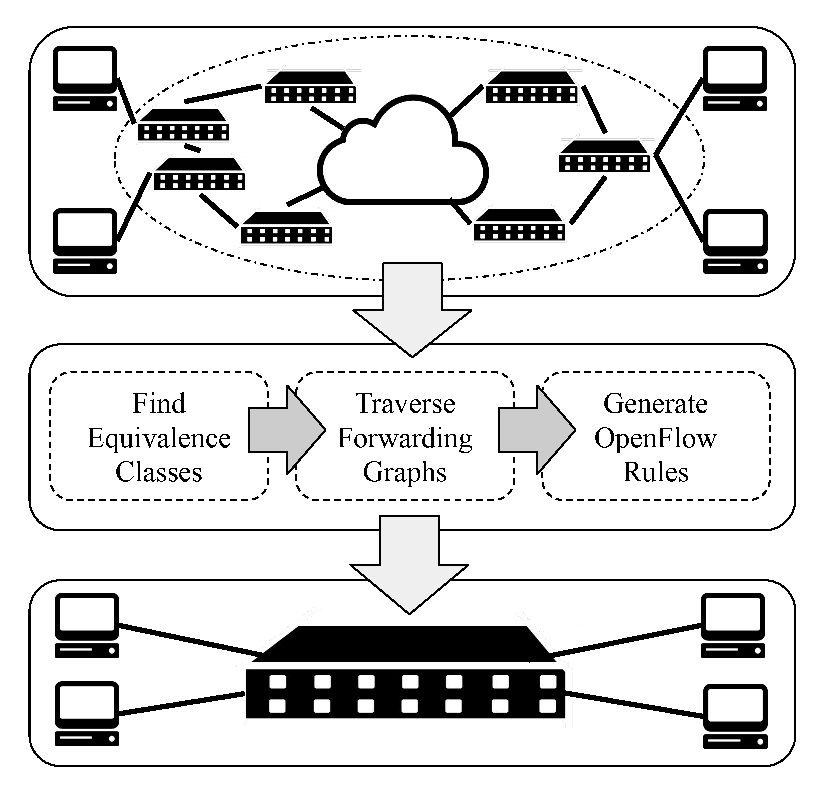
\includegraphics[width=0.9\textwidth]{OneBigSwitch/figures/BigSimOverview.eps}
\caption[One Big Switch Abstraction Overview]{Transforming an SDN network to a
    big OpenFlow switch based network while preserving the network forwarding logic equivalence.}
\label{OBS:Fig:BigSimOverview}
\end{figure}

The reduction in the number of switches and the number of rules significantly enhances the testbed scalability and reduces the experiment running time.
For example, after abstracting a tree-topology network of depth 4 and fanout 3,
the total number of switches required to simulate is reduced from 40 to 1, and the number of rules existed in the SDN network is reduced by 89\%.
The big-switch based network model can save about
75\% to 85\% simulation execution time as compared to simulating the original network.
We can also reuse the abstracted network model.
For example, after one complete experimental run of a complex network,
users can abstract (possibly part of) the network, and reproduce the simulation results with
a much simpler configuration, including link connectivity and flow tables.
We can partition a large-scale network model, and abstract each partition in parallel.
By combining those abstracted network models, a testing platform with limited hardware resources
now can afford such network simulation/emulation experiments.
As the network state evolves, the abstracted big-switch model may also need to be frequently updated.
Our approach is lightweight. For example, we can reduce 50,000+ rules in a large tree-topology network
to 5,000+ rules in a big-switch-based network in three seconds, 
while still preserving the network forwarding rule equivalence.
In addition, our approach allows incrementally updating the big-switch model,
i.e., modifying the rules that are only affected by the current network changes.

In this work, we present a model abstraction technique to reduce networked SDN switches to a one-big-switch model.
We mainly focus on preserving the end-to-end network forwarding logic.
Our long term goal is to investigate systematic model abstraction approaches that preserve end-to-end performance equivalence as well,
such as latency and packet drop, to further enhance the model fidelity.

The remainder of this paper is organized as follows.
Section~\ref{OBS:Sec:MotivatingExample} illustrates the problem and the approach using a simple motivating example.
Section~\ref{OBS:Sec:Design} describes the details of the three-step model abstraction design.
Section~\ref{OBS:Sec:Evaluation} presents the evaluation results in terms of forwarding logic equivalence, simulation time,
reduction in flow rules, and model abstraction execution time.
Section~\ref{OBS:Sec:relatedwork} summarizes the related works, and Section~\ref{OBS:Sec:conclusion} concludes the paper with future works.

\Section{Deep Learning Based Cyber Security System}
\label{DL:Sec:Intro}

Deep learning has gained a dramatic increase in popularity in the last couple of years,
and has offered advanced solutions in the areas of image and speech recognition~\cite{AlexNet, SpeechDNN},
natural language processing~\cite{Word2Vec}, Go playing~\cite{AlphaGo}, and many other domains~\cite{DeepLearning}. 
Motivated by deep learning's success, we ask what deep learning technology can do for cyber security.
Specifically, we focus on the domain of intrusion detection system.
Though both motivated by the deep learning technology, we have different answers for network-based and host-based intrusion detection systems respectively.


\Subsection{Deep Learning Based Network Intrusion Detection System}
\label{DL:SubSec:NIDS}
As networking technology gets deeply integrated into our lives, protecting modern networked systems against cyber-attacks is no longer optional.
Network intrusion detection systems (NIDSes) are essential security solutions for today's networked systems supporting military applications,
social communications, cloud services, and other critical infrastructures.
A NIDS automatically monitors traffic in a network to detect malicious activities and policy violations.
The majority of NIDSes today adopt signature-based detection techniques,
which can only identify known attacks via matching pre-installed signatures to observed network activities. 
The signature databases have to be frequently updated to include new types of attacks.
Those limitations have motivated researchers to investigate anomaly detection based approaches~\cite{STL-NIDS, LOF, RankingOutliner, NB-Tree, RampLossKSVCR, GAA-ADS}. 

Anomaly detection approaches use data mining or machine learning techniques to mathematically model the trustworthy network activities based on a set of training data,
and detect deviations from the model in observed data. A key advantage is the ability to detect unknown or novel malicious activities.
An on-line model further frees network administrators from identifying new patterns or even new types of the abnormal behaviors in a dynamic network environment.
However, if the constructed model is not sufficiently generalized for normal or abnormal traffic,
anomaly-based approaches would suffer from high false positive, i.e., incorrectly treat unknown normal traffic as malicious.

We study the feasibility of off-line deep learning based NIDS by constructing the detection engine with
multiple advanced deep learning models and conducting a quantitative and comparative evaluation of those models.
Specifically, we first introduce the general deep learning methodology and its potential implication on the network intrusion detection problem.
We then review multiple machine learning solutions to two network intrusion detection tasks (NSL-KDD and UNSW-NB15 datasets).
We develop a TensorFlow-based deep learning library, called NetLearner, and implement a handful of cutting-edge deep learning models for NIDS.
Finally, we conduct a quantitative and comparative performance evaluation of those models using NetLearner.



The remainder of this thesis is structured as follows.
Section~\ref{Sec:RelatedWork} briefly review the related work for each of the three topics.
Then Chapter 2 -- 4 discuss our proposed systems that address these topics in details,
typically in the order of: introducing motivation, describing system design,
then expermimental evaluation and final summary.
Chapter 5 concludes our work.
